\begin{figure}
    \centering
    

\tikzset{every picture/.style={line width=0.75pt}} %set default line width to 0.75pt        

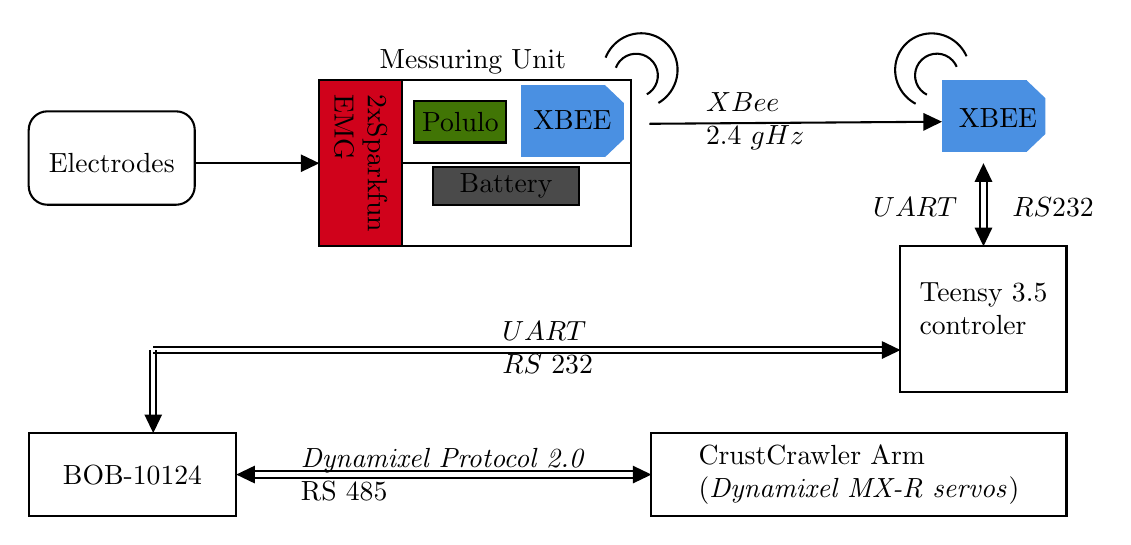
\begin{tikzpicture}[x=0.75pt,y=0.75pt,yscale=-1,xscale=1]
%uncomment if require: \path (0,278.7142848968506); %set diagram left start at 0, and has height of 278.7142848968506

%Rounded Rect [id:dp9198394438295476] 
\draw   (20,54) .. controls (20,49.03) and (24.03,45) .. (29,45) -- (91,45) .. controls (95.97,45) and (100,49.03) .. (100,54) -- (100,81) .. controls (100,85.97) and (95.97,90) .. (91,90) -- (29,90) .. controls (24.03,90) and (20,85.97) .. (20,81) -- cycle ;
%Straight Lines [id:da08300314610956905] 
\draw    (100,70) -- (158,70) ;
\draw [shift={(160,70)}, rotate = 540] [fill={rgb, 255:red, 0; green, 0; blue, 0 }  ][line width=0.75]  [draw opacity=0] (8.93,-4.29) -- (0,0) -- (8.93,4.29) -- cycle    ;

%Shape: Rectangle [id:dp49994760485296896] 
\draw   (160,30) -- (310,30) -- (310,110) -- (160,110) -- cycle ;
%Shape: Rectangle [id:dp9990642544965083] 
\draw  [fill={rgb, 255:red, 208; green, 2; blue, 27 }  ,fill opacity=1 ] (160,30) -- (200,30) -- (200,110) -- (160,110) -- cycle ;
%Straight Lines [id:da2266079205645528] 
\draw    (319,51) -- (458,50.01) ;
\draw [shift={(460,50)}, rotate = 539.5899999999999] [fill={rgb, 255:red, 0; green, 0; blue, 0 }  ][line width=0.75]  [draw opacity=0] (8.93,-4.29) -- (0,0) -- (8.93,4.29) -- cycle    ;

%Shape: Rectangle [id:dp7097032559017205] 
\draw   (200,30) -- (310,30) -- (310,70) -- (200,70) -- cycle ;
%Shape: Rectangle [id:dp16739603109917534] 
\draw   (200,70) -- (310,70) -- (310,110) -- (200,110) -- cycle ;
%Shape: Diagonal Stripe [id:dp825501516378429] 
\draw  [color={rgb, 255:red, 0; green, 0; blue, 0 }  ,draw opacity=0 ][fill={rgb, 255:red, 74; green, 144; blue, 226 }  ,fill opacity=1 ] (306.79,58.36) -- (297.73,67) -- (297.73,32.43) -- (306.79,41.07) -- cycle ;
%Shape: Rectangle [id:dp443446878421101] 
\draw  [draw opacity=0][fill={rgb, 255:red, 74; green, 144; blue, 226 }  ,fill opacity=1 ] (257,32.43) -- (297.73,32.43) -- (297.73,67) -- (257,67) -- cycle ;

%Shape: Rectangle [id:dp7890442898232035] 
\draw  [fill={rgb, 255:red, 74; green, 74; blue, 74 }  ,fill opacity=1 ] (215,72) -- (285,72) -- (285,90) -- (215,90) -- cycle ;
%Shape: Rectangle [id:dp3185767197775584] 
\draw  [fill={rgb, 255:red, 65; green, 117; blue, 5 }  ,fill opacity=1 ] (205.5,40) -- (250,40) -- (250,60) -- (205.5,60) -- cycle ;
%Shape: Arc [id:dp6014275798651711] 
\draw  [draw opacity=0] (302.89,23.99) .. controls (303.31,22.88) and (303.92,21.82) .. (304.74,20.86) .. controls (308.48,16.5) and (315.08,16.02) .. (319.46,19.79) .. controls (323.85,23.55) and (324.37,30.14) .. (320.63,34.5) .. controls (319.81,35.46) and (318.86,36.23) .. (317.82,36.8) -- (312.69,27.68) -- cycle ; \draw   (302.89,23.99) .. controls (303.31,22.88) and (303.92,21.82) .. (304.74,20.86) .. controls (308.48,16.5) and (315.08,16.02) .. (319.46,19.79) .. controls (323.85,23.55) and (324.37,30.14) .. (320.63,34.5) .. controls (319.81,35.46) and (318.86,36.23) .. (317.82,36.8) ;
%Shape: Arc [id:dp584505117797834] 
\draw  [draw opacity=0] (297.95,19.11) .. controls (298.69,17.23) and (299.75,15.44) .. (301.14,13.82) .. controls (307.69,6.19) and (319.05,5.19) .. (326.5,11.59) .. controls (333.96,17.98) and (334.69,29.36) .. (328.14,36.99) .. controls (326.75,38.61) and (325.14,39.94) .. (323.39,40.95) -- (314.64,25.4) -- cycle ; \draw   (297.95,19.11) .. controls (298.69,17.23) and (299.75,15.44) .. (301.14,13.82) .. controls (307.69,6.19) and (319.05,5.19) .. (326.5,11.59) .. controls (333.96,17.98) and (334.69,29.36) .. (328.14,36.99) .. controls (326.75,38.61) and (325.14,39.94) .. (323.39,40.95) ;

%Shape: Arc [id:dp9643215893864674] 
\draw  [draw opacity=0] (452.73,36.97) .. controls (451.67,36.44) and (450.68,35.71) .. (449.82,34.79) .. controls (445.9,30.59) and (446.15,23.98) .. (450.38,20.04) .. controls (454.61,16.09) and (461.21,16.3) .. (465.13,20.5) .. controls (465.99,21.42) and (466.65,22.46) .. (467.11,23.55) -- (457.48,27.65) -- cycle ; \draw   (452.73,36.97) .. controls (451.67,36.44) and (450.68,35.71) .. (449.82,34.79) .. controls (445.9,30.59) and (446.15,23.98) .. (450.38,20.04) .. controls (454.61,16.09) and (461.21,16.3) .. (465.13,20.5) .. controls (465.99,21.42) and (466.65,22.46) .. (467.11,23.55) ;
%Shape: Arc [id:dp6589182805450249] 
\draw  [draw opacity=0] (447.33,41.35) .. controls (445.55,40.4) and (443.88,39.15) .. (442.42,37.58) .. controls (435.56,30.23) and (435.82,18.84) .. (443.01,12.13) .. controls (450.19,5.43) and (461.58,5.96) .. (468.44,13.31) .. controls (469.9,14.88) and (471.03,16.63) .. (471.85,18.47) -- (455.43,25.45) -- cycle ; \draw   (447.33,41.35) .. controls (445.55,40.4) and (443.88,39.15) .. (442.42,37.58) .. controls (435.56,30.23) and (435.82,18.84) .. (443.01,12.13) .. controls (450.19,5.43) and (461.58,5.96) .. (468.44,13.31) .. controls (469.9,14.88) and (471.03,16.63) .. (471.85,18.47) ;

%Straight Lines [id:da8446148813559833] 
\draw    (481.5,78) -- (481.5,102)(478.5,78) -- (478.5,102) ;
\draw [shift={(480,110)}, rotate = 270] [fill={rgb, 255:red, 0; green, 0; blue, 0 }  ][line width=0.75]  [draw opacity=0] (8.93,-4.29) -- (0,0) -- (8.93,4.29) -- cycle    ;
\draw [shift={(480,70)}, rotate = 90] [fill={rgb, 255:red, 0; green, 0; blue, 0 }  ][line width=0.75]  [draw opacity=0] (8.93,-4.29) -- (0,0) -- (8.93,4.29) -- cycle    ;
%Straight Lines [id:da5044267925519024] 
\draw    (432,161.5) -- (80,161.5)(432,158.5) -- (80,158.5) ;

\draw [shift={(440,160)}, rotate = 180] [fill={rgb, 255:red, 0; green, 0; blue, 0 }  ][line width=0.75]  [draw opacity=0] (8.93,-4.29) -- (0,0) -- (8.93,4.29) -- cycle    ;
%Straight Lines [id:da7406026285596496] 
\draw    (81.5,160) -- (81.5,192)(78.5,160) -- (78.5,192) ;
\draw [shift={(80,200)}, rotate = 270] [fill={rgb, 255:red, 0; green, 0; blue, 0 }  ][line width=0.75]  [draw opacity=0] (8.93,-4.29) -- (0,0) -- (8.93,4.29) -- cycle    ;

%Shape: Rectangle [id:dp016623272212034745] 
\draw   (20,200) -- (120,200) -- (120,240) -- (20,240) -- cycle ;
%Straight Lines [id:da7263406511929] 
\draw    (128,218.5) -- (312,218.5)(128,221.5) -- (312,221.5) ;
\draw [shift={(320,220)}, rotate = 180] [fill={rgb, 255:red, 0; green, 0; blue, 0 }  ][line width=0.75]  [draw opacity=0] (8.93,-4.29) -- (0,0) -- (8.93,4.29) -- cycle    ;
\draw [shift={(120,220)}, rotate = 0] [fill={rgb, 255:red, 0; green, 0; blue, 0 }  ][line width=0.75]  [draw opacity=0] (8.93,-4.29) -- (0,0) -- (8.93,4.29) -- cycle    ;
%Shape: Rectangle [id:dp6457555540924869] 
\draw   (320,200) -- (520,200) -- (520,240) -- (320,240) -- cycle ;
%Shape: Diagonal Stripe [id:dp03884391194674164] 
\draw  [color={rgb, 255:red, 0; green, 0; blue, 0 }  ,draw opacity=0 ][fill={rgb, 255:red, 74; green, 144; blue, 226 }  ,fill opacity=1 ] (509.79,55.93) -- (500.73,64.57) -- (500.73,30) -- (509.79,38.64) -- cycle ;
%Shape: Rectangle [id:dp43104363535705037] 
\draw  [draw opacity=0][fill={rgb, 255:red, 74; green, 144; blue, 226 }  ,fill opacity=1 ] (460,30) -- (500.73,30) -- (500.73,64.57) -- (460,64.57) -- cycle ;
%Shape: Rectangle [id:dp6427493868255278] 
\draw   (440,110) -- (520,110) -- (520,180) -- (440,180) -- cycle ;

% Text Node
\draw (60,70) node  [align=left] {Electrodes};
% Text Node
\draw (234,21) node  [align=left] {Messuring Unit};
% Text Node
\draw (282,49) node  [align=left] {XBEE};
% Text Node
\draw (250,81) node  [align=left] {Battery};
% Text Node
\draw (180,70) node [rotate=-90] [align=left] {2xSparkfun \\EMG};
% Text Node
\draw (228,50) node  [align=left] {Polulo};
% Text Node
\draw (70,220) node  [align=left] {BOB-10124};
% Text Node
\draw (220,220) node  [align=left] {\textit{Dynamixel Protocol 2.0}\\RS 485};
% Text Node
\draw (420,220) node  [align=left] {CrustCrawler Arm\\(\textit{Dynamixel MX-R servos})};
% Text Node
\draw (370,50) node   {$ \begin{array}{l}
XBee\\
2.4\ gHz
\end{array}$};
% Text Node
\draw (480,140) node  [align=left] {Teensy 3.5\\controler};
% Text Node
\draw (480,91) node   {$UART\ \ \ \ \ \ RS232$};
% Text Node
\draw (270,160) node   {$ \begin{array}{l}
UART\\
RS\ 232
\end{array}$};
% Text Node
\draw (487,48) node  [align=left] {XBEE};


\end{tikzpicture}

    \caption{Illustration of the specific solution used. Arrows show the direction data is send, and boxes have the specific name of the module used. Note a few changes from Figure \ref{fig:GenDesign}. italic text shows the hardware used to send a specific protocol}
    \label{fig:SpecificDesign}
\end{figure}